\chapter{Budowa i działanie systemu GGSS}
\label{cha:ggss}

Niniejszy rozdział zawiera ważne, z punktu widzenia przeprowadzonych prac, informacje na temat systemu GGSS. Przedstawione tu opisy dotyczą zagadnień takich jak: wysokopoziomowa architektura systemu, struktura warstwy oprogramowania, opis wykorzystywanych przez system urządzeń oraz omówienie cech charakterystycznych środowiska docelowego. 


\section{Wysokopoziomowa architektura systemu GGSS}
System GGSS składa się z kilku współpracujących ze sobą elementów, przedstawionych (wraz z występującymi między nimi interakcjami) na rysunku \ref{fig:high_level_architecture}. Znaczenie poszczególnych komponentów projektu jest następujące:
\begin{itemize}
    \item \textbf{oprogramowanie GGSS} - zestaw aplikacji wraz z otaczającą je infrastrukturą, których zadaniem jest sterowanie urządzeniami wchodzącymi w skład systemu GGSS oraz przetwarzanie zbieranych za ich pomocą danych
    \item \textbf{urządzenia (ang. \textit{hardware})} - zestaw urządzeń elektronicznych (m.in. liczniki słomkowe, zasilacze wysokiego napięcia i multipleksery)
    \item \textbf{pliki konfiguracyjne} - proste pliki tekstowe w formacie XML \textbf{rozwin + cytowanie}, zawierające informacje o oczekiwanym sposobie działania systemu (np. maksymalna możliwa wartość napięcia, jakie może zostać ustawione na każdym z zasilaczy)
    \item \textbf{pliki wynikowe} - pliki tekstowe zawierające wyniki pomiarów wykonywanych przez system oraz rejestr zdarzeń 
    \item \textbf{system WinCC OA} - \textbf{rozwin + cytowanie} - system typu SCADA \textbf{rozwin + cytowanie}, stanowiący część systemu kontroli detektora ATLAS (DCS), pozwalający na obserwację i kontrolę działania poszczególnych poddetektorów
    \item \textbf{protokół DIM} - \textbf{rozwin + cytowanie} protokół komunikacyjny dla środowisk rozproszonych, oparty o architekturę klient-serwer, zapewniający komunikację między oprogramowaniem systemu GGSS a systemem WinCC OA
\end{itemize}

\begin{figure}[H]
\centering
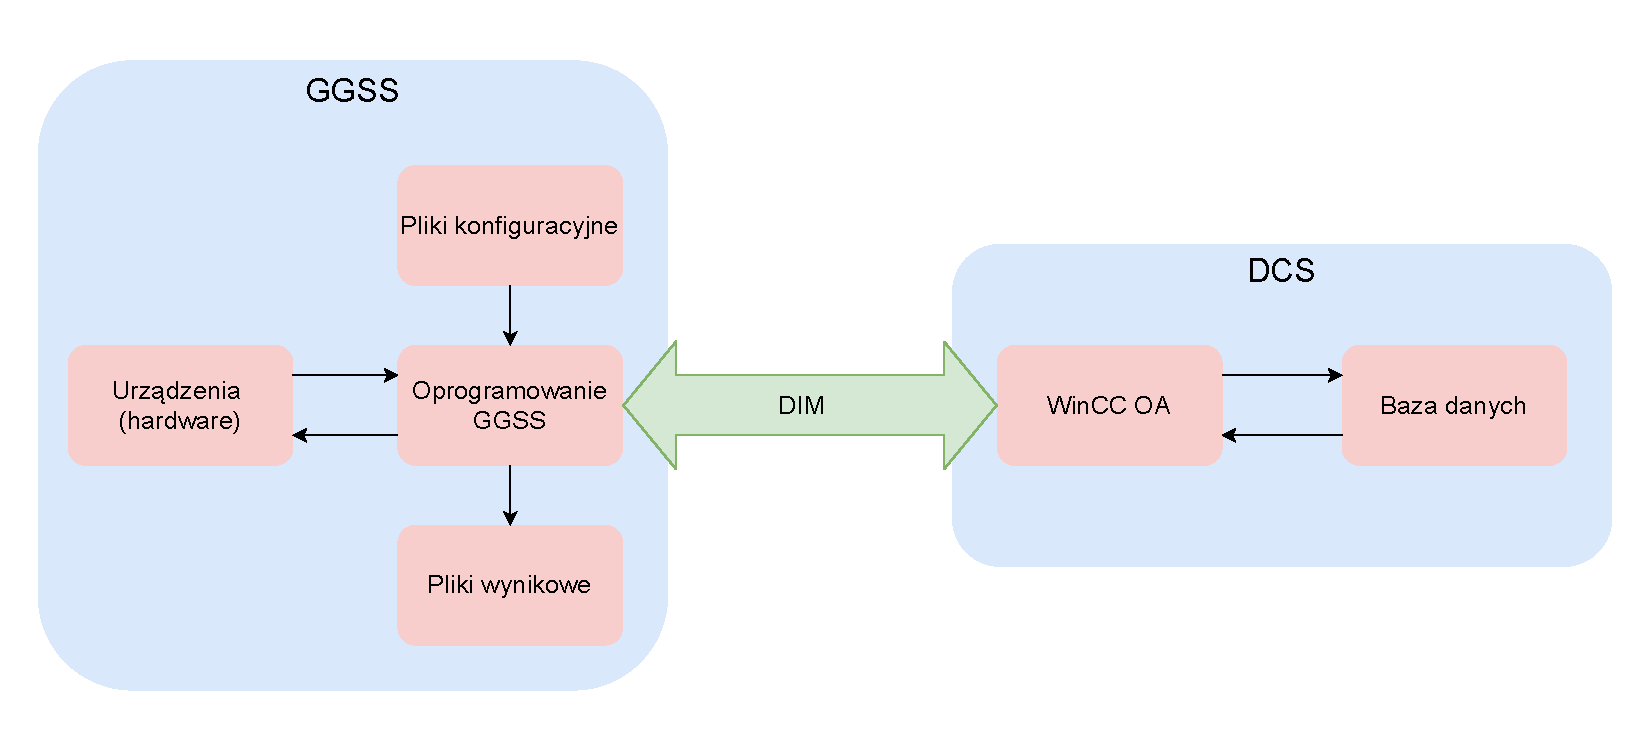
\includegraphics[width=\textwidth]{components/ggss_images/high_level_architecture.pdf}
\caption{Wysokopoziomowa architektura projektu GGSS. Strzałkami oznaczono przepływ danych pomiędzy poszczególnymi komponentami systemu.}
\label{fig:high_level_architecture}
\end{figure}


Szczegóły działania najważniejszych z punktu widzenia niniejszej pracy elementów systemu omówione zostaną w dalszej części tego rozdziału. Znaczna część prac opisanych w niniejszym manuskrypcie skupiona była na udoskonaleniu warstwy oprogramowania systemu GGSS.


\section{Urządzenia elektroniczne}
Z punktu widzenia warstwy sprzętowej system GGSS składa się z zestawu tzw. słomkowych liczników proporcjonalnych, zasilanych za pomocą zasilaczy wysokiego napięcia. Sygnały generowane przez liczniki przetwarzane są przez wielokanałowy analizator amplitudy (MCA - \textbf{rozwinac}), natomiast wybór licznika słomkowego używanego do wykonania pomiarów następuje za pomocą multipleksera analogowego \textbf{cytowanie}. Urządzenia podłączone są do komputera PC, który steruje nimi za pomocą oprogramowania systemu GGSS. W tabeli \ref{tab:devices} zamieszczone zostało zestawienie informacji na temat wykorzystywanych przez projekt urządzeń. Sposób działania systemu (jego podstawa fizyczna oraz znaczenie przeprowadzanych pomiarów) wykracza poza zakres niniejszej pracy, został natomiast szczegółowo opisany w pracy \emph{Wybrane zagadnienia związane z pracą słomkowych liczników proporcjonalnych w detektorze TRT eksperymentu ATLAS}, której autorem jest dr hab. inż. Bartosz Mindur, prof. AGH \textbf{cytowanie}.

\clearpage

\begin{table*}[htbp]
\centering
\caption{Zestawienie istotnych z punktu widzenia niniejszej pracy urządzeń wchodzących w skład systemu GGSS.}
\label{tab:devices}
\begin{tabularx}{\textwidth}{@{}XX@{}}
\toprule
Urządzenie &
Informacje \\
\midrule
4-kanałowy zasilacz wysokiego napięcia & CAEN N1470 \\
wielokanałowy analizator amplitudy & CAEN N957 \\
multiplekser sygnałów analogowych & urządzenie autorstwa Pana Pawła Zadrożniaka\\
\bottomrule
\end{tabularx}
\end{table*}


\section{Warstwa oprogramowania}
Poprzez warstwę oprogramowania systemu GGSS autorzy rozumieją zarówno zestaw aplikacji napisanych w języku C++ (standard 11), jak i otaczającą je infrastrukturę (pomocnicze skrypty, system budowania, testowania i tworzenia nowych wydań). 



\subsection{Aplikacje wchodzące w skład GGSS}
Trzon warstwy oprogramowania projektu GGSS stanowi aplikacja \emph{ggss-runner}, zawierająca logikę odpowiedzialną za komunikację z systemem za pomocą protokołu DIM, gromadzenie i walidację danych oraz sterowanie urządzeniami wchodzącymi w skład warstwy sprzętowej. W skład systemu wchodzi ponadto szereg pomniejszych aplikacji (niektóre z nich stanowią element dodany przez autorów niniejszej pracy, zostaną więc omówione ze szczegółami w dalszych jej częściach):
\begin{itemize}
    \item \emph{ggss-spector} - aplikacja okienkowa służąca do wizualizacji zebranych przez system danych (zapisanych w plikach wynikowych)
    \item \emph{ggss-reader} - niezależna aplikacja przeznaczona do wykorzystywania na maszynach deweloperskich, pozwalająca na odtwarzanie działania oprogramowania sterującego GGSS, tzn. wysyłająca do systemu kontroli detektora archiwalne dane z pominięciem warstwy sprzętowej \textbf{cytowanie pracy grzeska}
    \item \emph{ggss-dim-cs} - aplikacja pozwalająca na wysyłanie do systemu komend za pomocą protokołu DIM \textbf{tutaj cytowanie}
    \item zestaw aplikacji \emph{ggss-hardware-service-apps} - proste narzędzia pozwalające na wykonywanie operacji na wchodzących w skład systemu urządzaniach, w tym na wykonywanie testów ich działania. 
\end{itemize}


\subsection{Język C++}
Zarówno aplikacja \emph{ggss-runner}, jak i wszystkie aplikacje pomocnicze, napisane zostały za pomocą języka C++. Jest to wydajny, wszechstronny język programowania ogólnego przeznaczenia, pozwalający programiście zarówno na wykorzystywanie wysokopoziomowych abstrakcji (programowanie obiektowe, generyczne i funkcyjne), jak i na wydajne wykonywanie niskopoziomowych operacji. W ciągu ostatnich dziesięciu lat język ten był intensywnie rozwijany - od 2011 roku pojawiły się cztery nowe standardy, w tym najnowszy w roku 2020, a kolejny przewidziany jest na rok 2023. Zmiany wprowadzane w nowych wydaniach języka mają na celu zarówno dodawanie do niego nowych funkcjonalności, jak równeż promowanie praktych pozwalających tworzyć prosty w utrzymaniu, czytelny kod. Niestety z uwagi na ograniczenia wynikające ze cech środowiska docelowego, w jakim działać ma system GGSS, w omawianym projekcie możliwe było wykorzystanie jedynie standardu C++11. 


\subsection{Biblioteki zewnętrzne}
W projekcie wykorzystywane są ponadto biblioteki nie będące częścią standardu języka C++, dostarczające funkcjonalności niezbędnych do poprawnego działania systemu. Najważniejsze z nich to:
\begin{itemize}
    \item \emph{Boost} \textbf{cytowanie} - rozbudowany zestaw bibliotek dla języka C++, cieszący się znaczącą popularnością, m.in. ze względu na wysoką jakość i szeroki zakres wprowadzanych funkcjonalności (m.in. przetwarzanie argumentów linii poleceń, implementacja operacji na grafach, wsparcie dla programowania sieciowego, tworzenia testów jednostkowych czy zaawansowanego metaprogramowania). Ponadto niektóre z bibliotek wchodzących w skład \emph{Boost} były podstawą do implementacji funkcjonalności takich jak inteligentne wskaźniki (ang. smart pointers) czy obsługa wyrażeń regularnych w nowych standardach języka C++.
    \item \emph{GNU Scientific Library (GSL)} \textbf{cytowanie} - biblioteka dla języków C i C++, dostarczająca implementacje popularnych algorytmów numerycznych
    \item \emph{Qt} oraz \emph{Qwt} \textbf{cytowanie} - wieloplatformowy zestaw bibliotek i narzędzi pozwalających na tworzenie aplikacji okienkowych, wykorzystywany przez aplikacje \emph{ggss-spector} oraz \emph{ggss-reader}
    \item \emph{DIM} \textbf{cytowanie} - dostarczona przez CERN biblioteka umożliwiająca wykorzystywanie protokołu DIM
    \item \emph{CAEN-N957} \textbf{cytowanie} - dostarczona przez firmę CAEN biblioteka współdzielona napisana w języku C, służąca do obsługi analizatora wielokanałowego N957
\end{itemize}


\subsection{Infrastruktura projektu}
Projekt GGSS charakteryzuje się rozbudowaną infrastrukturą, w której skład wchodzą systemy odpowiedzialne za budowanie projektu, zarządzanie zależnościami pomiędzy jego komponentami (również wewnątrz samego projektu), automatyzację procesu testowania poszczególnych komponentów oraz automatyzację tworzenia i wersjonowania wydań. Ponadto w jej skład wchodzą skrypty pomocnicze (napisane w językach Bash \textbf{cytat} i Python \textbf{cytat}), pozwalające na zarządzanie systemem w jego środowisku docelowym. Gruntowna przebudowa infrastruktury systemu GGSS stanowiła temat pracy inżynierskiej autorów (\textbf{cytat i tytul}). W dalszej części niniejszego manuskryptu omówione zostaną wprowadzone w ramach pracy magistersiej rozszerzenia. 

Infrastruktura budowania projektu oparta jest o narzędzie CMake (\textbf{cytowanie}) (wersja 2.8) rozwijane przez firmę \emph{Kitware}. Zastosowanie go pozwala na generowanie pliku budującego projekt właściwego dla danej platformy docelowej (np. \emph{Makefile} dla systemów z rodziny UNIX), a co za tym idzie, pozwala na łatwe tworzenie aplikacji wieloplatformowych. Stosując narzędzie CMake, tworzenie systemu budowania projektu polega na przygotowaniu pliku (lub zestawu plików) \emph{CMakeLists.txt}, zawierającego polecenia pozwalające na określenie przez programistę informacji takich jak: standard języka C++, lokalizacja plików źródłowych i bibliotek zewnętrznych.

\section{Oprogramowanie WinCC OA}
SIMATIC WinCC Open Architecture jest oprogramowaniem typu SCADA firmy SIEMENS służącym do wizualizacji i sterowania procesami produkcyjnymi. System ten stanowi trzon systemu kontroli detektora ATLAS (DCS) i pozwala na monitorowanie i sterowanie pracą wchodzących w jego skład podsystemów. WinCC OA pozwala m.in. na tworzenie specjalnych paneli, obrazujacych zebrane dane oraz procesy zachodzące w monitorowanym systemie - przykład tego typu panelu, obrazujący pracę liczników słomkowych wykorzystywanych przez GGSS, przedstawiony został na rysunku \ref{fig:winccoa_panel_example}.

(https://new.siemens.com/global/en/products/automation/industry-software/automation-software/scada/simatic-wincc-oa/wincc-oa-basic-software.html)


W ramach pracy magisterskiej autorzy nie wykonywali żadnych prac związanych z rozwojem czy utrzymaniem oprogramowania WinCC OA. Jest ono natomiast szczególnie istotne z punktu widzenia testów, jakim musiał być poddawany system GGSS wraz z postępami prac. \textbf{dopisac dlaczego, napisac cos jeszcze moze np o pracy grzeska}

% Krotko co to jest
% Co to sa panele, pokazac przyklad
% Krotko jak dziala DIM, co jest u nas klientem, a co serwerem

\begin{figure}[H]
\centering
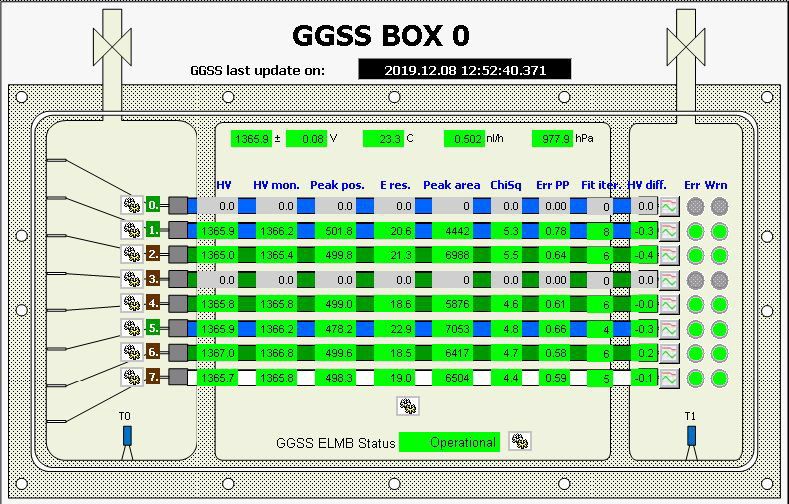
\includegraphics[width=\textwidth]{components/ggss_images/winccoa_panel.png}
\caption{}
\label{fig:winccoa_panel_example}
\end{figure}

\section{Środowisko docelowe i ograniczenia}
Charakterystyka środowiska docelowego, w jakim działa system GGSS, jest z punktu widzenia niniejszej pracy bardzo istotna - silny związek projektu z infrastrukturą dostarczaną przez CERN stawia przed autorami niniejszej pracy szereg ograniczeń dotyczących wersji wykorzystywanych narzędzi, jak również wymusza dodatkowe działania w przypadku wykonywania pewnych operacji. Do najważniejszych ograniczeń narzucanych przez środowisko docelowe i specyfikę projektu należą:
\begin{itemize}
    \item dostępna wersje kompilatora języka C++ - w ramach infrastruktury CERN dostępny jest kompilator \emph{g++ (GCC) 4.8.5}. Wersja ta wspiera w większości standard C++11, a zatem funkcjonalności takie jak wyrażenia lambda czy semantyka przenoszenia. Niestety oferowane przez nią wsparcie nie jest pełne - brakuje m.in. poprawnej implementacji biblioteki odpowiedzialnej za przetwarzanie wyrażeń regularnych. Ze względu na wymóg zapewnienia możliwości budowania projektu na maszynie docelowej, ograniczenie to stanowiło znaczące utrudnienie podczas prac nad kodem źródłowym aplikacji wchodzących w skład systemu.
    \item dostępna wersja narzędzia CMake - na maszynach docelowych dostępna jest wersja \emph{2.8.12.2}, stanowiąca bardzo stare wydanie narzędzia. \textbf{dopisac cos}
    \item związek projektu z wersją jądra systemu \textbf{dopisac cos}
    \item możliwość przeprowadzania testów tylko w określonych momentach prac nad projektem \textbf{dopisac cos}
    \item ograniczone uprawnienia w środowisku docelowym \textbf{dopisac cos}
    \item konieczność zachowania kompatybilności wstecznej \textbf{dopisac cos}
\end{itemize}



% Dedykowany komputer
% Jakie ograniczenia wynikaja z tego
% Wymog wstecznej kompatybilnosci
